% Created by tikzDevice version 0.10.1 on 2016-04-19 18:05:39
% !TEX encoding = UTF-8 Unicode
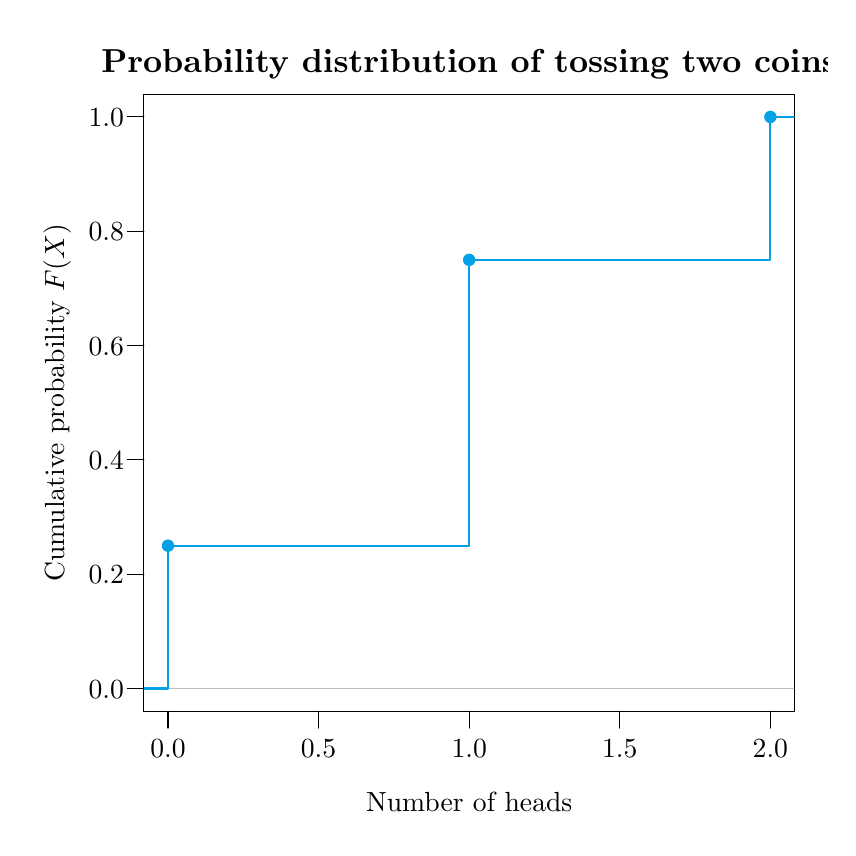
\begin{tikzpicture}[x=1pt,y=1pt]
\definecolor{fillColor}{RGB}{255,255,255}
\path[use as bounding box,fill=fillColor,fill opacity=0.00] (0,0) rectangle (289.08,289.08);
\begin{scope}
\path[clip] ( 42.00, 42.00) rectangle (277.08,265.08);
\definecolor{fillColor}{RGB}{5,161,230}

\path[fill=fillColor] ( 50.71,101.90) circle (  2.25);

\path[fill=fillColor] (159.54,205.18) circle (  2.25);

\path[fill=fillColor] (268.37,256.82) circle (  2.25);
\end{scope}
\begin{scope}
\path[clip] (  0.00,  0.00) rectangle (289.08,289.08);
\definecolor{drawColor}{RGB}{0,0,0}

\path[draw=drawColor,line width= 0.4pt,line join=round,line cap=round] ( 50.71, 42.00) -- (268.37, 42.00);

\path[draw=drawColor,line width= 0.4pt,line join=round,line cap=round] ( 50.71, 42.00) -- ( 50.71, 36.00);

\path[draw=drawColor,line width= 0.4pt,line join=round,line cap=round] (105.12, 42.00) -- (105.12, 36.00);

\path[draw=drawColor,line width= 0.4pt,line join=round,line cap=round] (159.54, 42.00) -- (159.54, 36.00);

\path[draw=drawColor,line width= 0.4pt,line join=round,line cap=round] (213.96, 42.00) -- (213.96, 36.00);

\path[draw=drawColor,line width= 0.4pt,line join=round,line cap=round] (268.37, 42.00) -- (268.37, 36.00);

\node[text=drawColor,anchor=base,inner sep=0pt, outer sep=0pt, scale=  1.00] at ( 50.71, 25.20) {0.0};

\node[text=drawColor,anchor=base,inner sep=0pt, outer sep=0pt, scale=  1.00] at (105.12, 25.20) {0.5};

\node[text=drawColor,anchor=base,inner sep=0pt, outer sep=0pt, scale=  1.00] at (159.54, 25.20) {1.0};

\node[text=drawColor,anchor=base,inner sep=0pt, outer sep=0pt, scale=  1.00] at (213.96, 25.20) {1.5};

\node[text=drawColor,anchor=base,inner sep=0pt, outer sep=0pt, scale=  1.00] at (268.37, 25.20) {2.0};

\path[draw=drawColor,line width= 0.4pt,line join=round,line cap=round] ( 42.00, 50.26) -- ( 42.00,256.82);

\path[draw=drawColor,line width= 0.4pt,line join=round,line cap=round] ( 42.00, 50.26) -- ( 36.00, 50.26);

\path[draw=drawColor,line width= 0.4pt,line join=round,line cap=round] ( 42.00, 91.57) -- ( 36.00, 91.57);

\path[draw=drawColor,line width= 0.4pt,line join=round,line cap=round] ( 42.00,132.88) -- ( 36.00,132.88);

\path[draw=drawColor,line width= 0.4pt,line join=round,line cap=round] ( 42.00,174.20) -- ( 36.00,174.20);

\path[draw=drawColor,line width= 0.4pt,line join=round,line cap=round] ( 42.00,215.51) -- ( 36.00,215.51);

\path[draw=drawColor,line width= 0.4pt,line join=round,line cap=round] ( 42.00,256.82) -- ( 36.00,256.82);

\node[text=drawColor,anchor=base east,inner sep=0pt, outer sep=0pt, scale=  1.00] at ( 34.80, 46.82) {0.0};

\node[text=drawColor,anchor=base east,inner sep=0pt, outer sep=0pt, scale=  1.00] at ( 34.80, 88.13) {0.2};

\node[text=drawColor,anchor=base east,inner sep=0pt, outer sep=0pt, scale=  1.00] at ( 34.80,129.44) {0.4};

\node[text=drawColor,anchor=base east,inner sep=0pt, outer sep=0pt, scale=  1.00] at ( 34.80,170.75) {0.6};

\node[text=drawColor,anchor=base east,inner sep=0pt, outer sep=0pt, scale=  1.00] at ( 34.80,212.06) {0.8};

\node[text=drawColor,anchor=base east,inner sep=0pt, outer sep=0pt, scale=  1.00] at ( 34.80,253.37) {1.0};

\path[draw=drawColor,line width= 0.4pt,line join=round,line cap=round] ( 42.00, 42.00) --
	(277.08, 42.00) --
	(277.08,265.08) --
	( 42.00,265.08) --
	( 42.00, 42.00);
\end{scope}
\begin{scope}
\path[clip] (  0.00,  0.00) rectangle (289.08,289.08);
\definecolor{drawColor}{RGB}{0,0,0}

\node[text=drawColor,anchor=base,inner sep=0pt, outer sep=0pt, scale=  1.20] at (159.54,272.89) {\bfseries Probability distribution of tossing two coins};

\node[text=drawColor,anchor=base,inner sep=0pt, outer sep=0pt, scale=  1.00] at (159.54,  6.00) {Number of heads};

\node[text=drawColor,rotate= 90.00,anchor=base,inner sep=0pt, outer sep=0pt, scale=  1.00] at ( 13.20,153.54) {Cumulative probability $F(X)$};
\end{scope}
\begin{scope}
\path[clip] ( 42.00, 42.00) rectangle (277.08,265.08);
\definecolor{drawColor}{RGB}{190,190,190}

\path[draw=drawColor,line width= 0.4pt,line join=round,line cap=round] ( 42.00, 50.26) -- (277.08, 50.26);
\definecolor{drawColor}{RGB}{5,161,230}

\path[draw=drawColor,line width= 0.8pt,line join=round,line cap=round] (  0.00, 50.26) --
	( 50.71, 50.26) --
	( 50.71,101.90) --
	(159.54,101.90) --
	(159.54,205.18) --
	(268.37,205.18) --
	(268.37,256.82) --
	(289.08,256.82);
\end{scope}
\end{tikzpicture}
